\section{Results}
\label{sec:results}

\subsection{Inferred velocities}

Figure \ref{fig:results} shows the inferred velocities of 5000 randomly
selected Kepler stars.
The 2D distributions of inferred stellar velocities are plotted in the
lower-left panels, with black contours indicating the stellar number density.
The red contours in these panels show the marginal projections of the
Gaussian prior in 2D.
The diagonal panels show the 1D distributions (histograms) of stellar
velocities.
The black histogram shows the distribution of inferred velocities, the cyan
histogram shows the distribution of velocities calculated for stars with RVs,
and the red lines show the 1D marginal Gaussian prior distributions.
This figure shows that the velocity distributions of stars calculated with and
without RVs are broadly similar.
The prior distribution is calculated using the velocities of stars with RVs.
If the velocity distributions of stars were Gaussian, the 1D red Gaussians
would look like the cyan histograms.
In other words, the differences between the red lines and cyan histograms
is caused by the non-Gaussianity of the velocity distributions.

Among stars with measured RVs, \vy\ and \vz\ are slightly positively
correlated: stars with larger \vy\ tend to have larger \vz.
However, the inferred velocities have the opposite trend: stars with larger
\vy\ have a smaller \vz.
This difference is caused by the slight degeneracy between \vy\ and \vz\ for
stars that do not have RVs.
The proper motions of stars with a given \vy\ and \vz\ could be equally
well-described with a slightly larger \vy\ and a smaller \vz\ or vice versa.

\begin{figure}[ht!]
\caption{
The distribution of inferred stellar velocities and distances.
    Figure \ref{fig:results} shows the inferred velocities of 5000 randomly
selected Kepler stars.
The 2D distributions of inferred stellar velocities are plotted in the
lower-left panels, with black contours indicating the stellar number density.
The orange contours in the lower-left panels show the marginal projections of
    the Gaussian prior distribution in 2D.
The upper-right panels in the figure, lying on the plot's diagonal, show the
    1D distributions (histograms) of stellar velocities.
The black histogram shows the distribution of inferred velocities, the blue
histogram shows the distribution of velocities for stars with RVs,
and the orange lines show the 1D marginal Gaussian prior distributions.
}
  \centering
    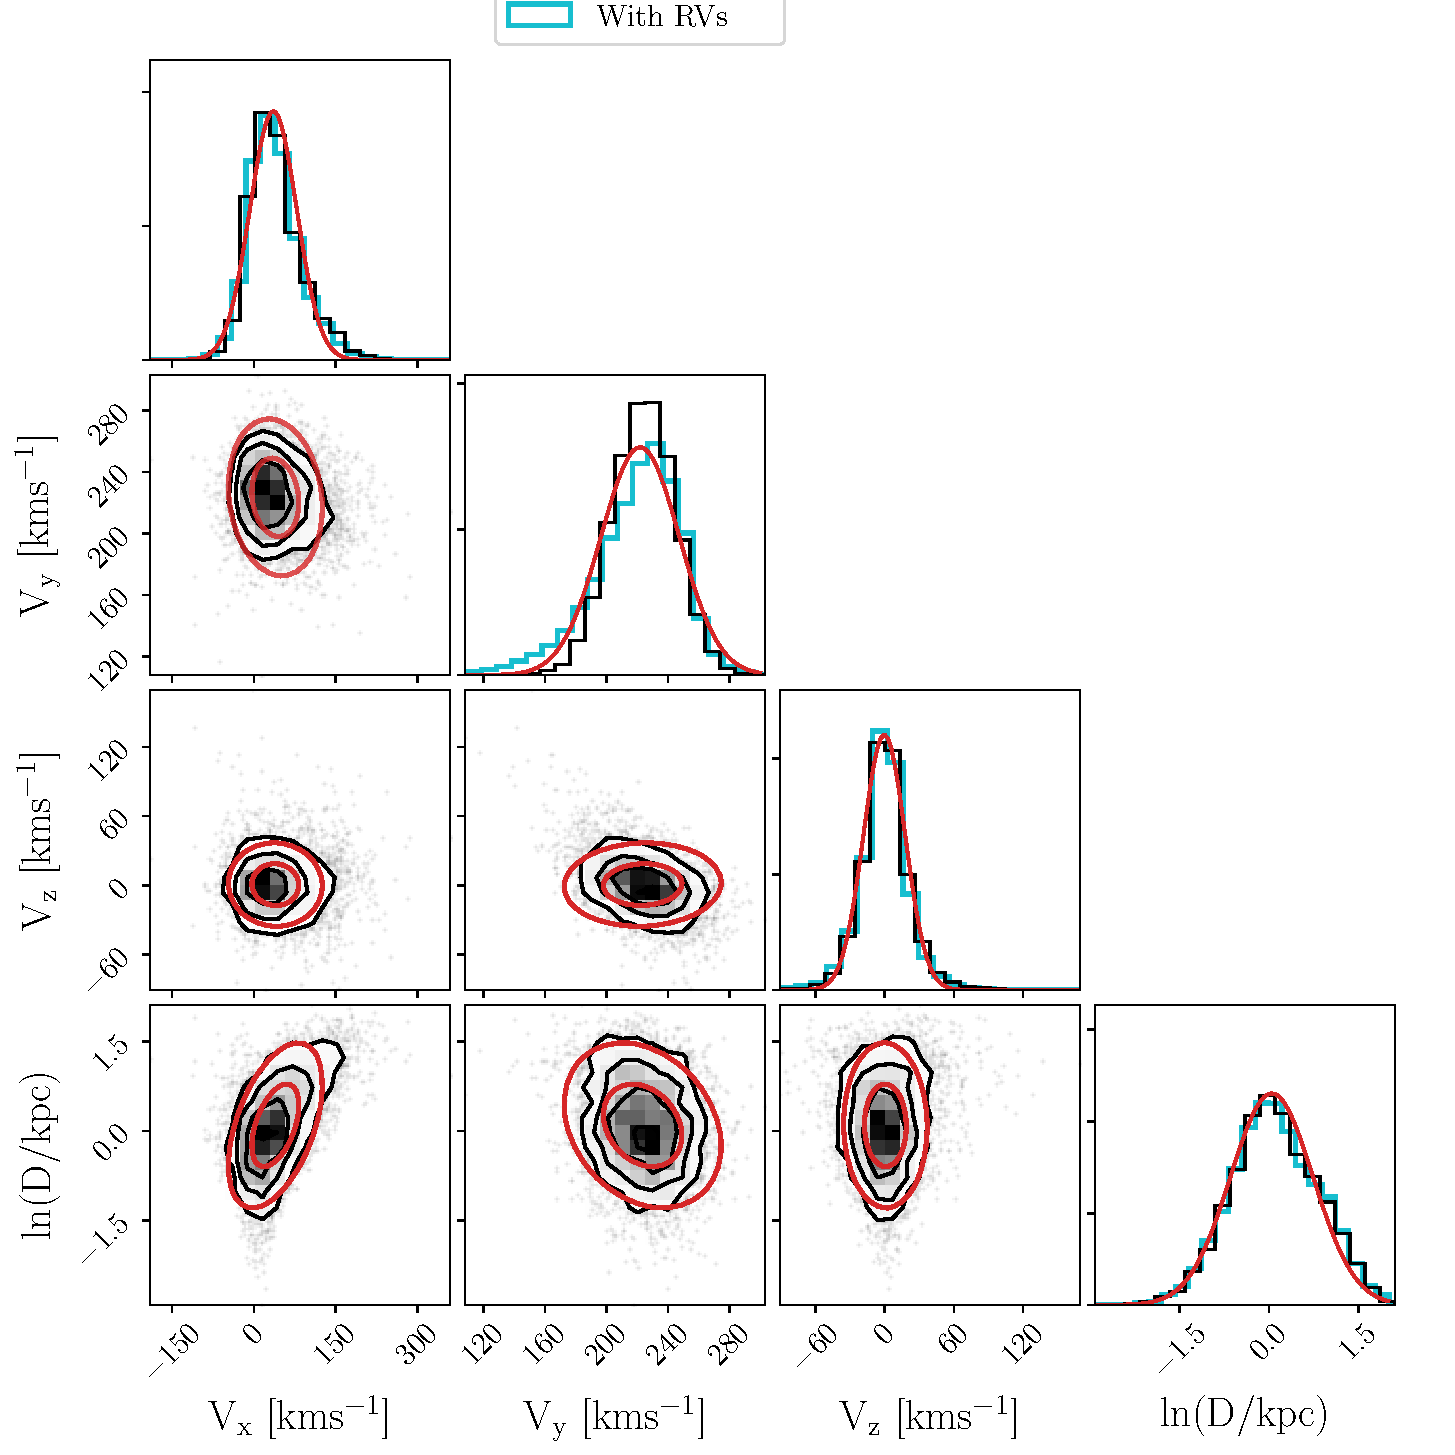
\includegraphics[width=1\textwidth]{results}
\label{fig:results}
\end{figure}


To validate our method, we inferred velocities for stars in our sample with
measured RVs and compared those inferred values with velocities calculated
directly from 6D position, proper motion, and RV measurements.
Figure \ref{fig:residuals} shows the \vx, \vy\ and \vz\ velocities we
inferred, for 3000 stars chosen at random, compared with those calculated from
measured RVs.
\begin{figure}[ht!]
\caption{Vertical velocities calculated with full 6D information vs vertical
    velocities inferred without RVs, for 3000 Kepler targets with RV
    measurements.}
  \centering
    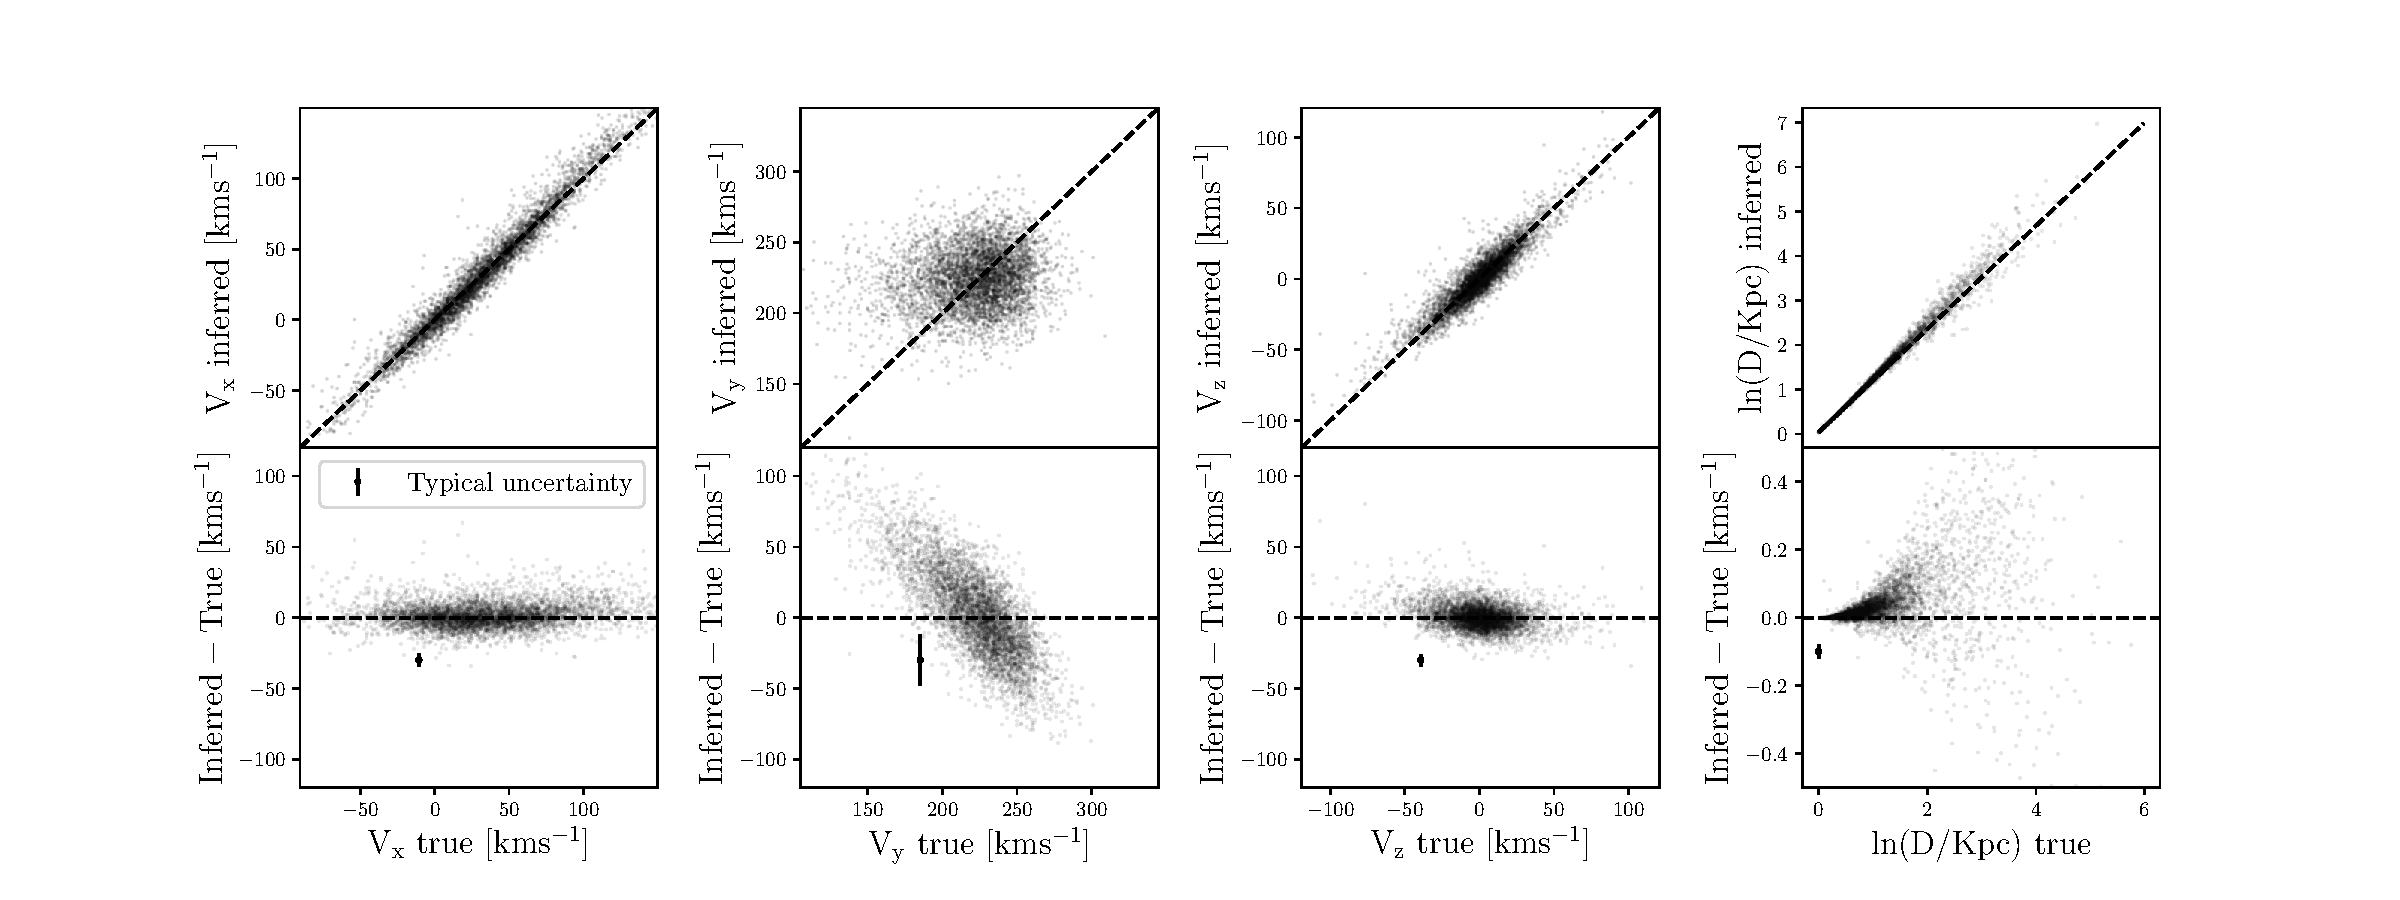
\includegraphics[width=1\textwidth]{residuals}
\label{fig:residuals}
\end{figure}

The three velocity components, \vx, \vy\ and \vz\ were recovered with
differing levels of precision: \vx\ and \vz\ are inferred more precisely than
\vy.
This is because of the orientation of the \kepler\ field, shown in figure
\ref{fig:kepler_field}.
\racomment{Slight inaccuracies seen in the residual panels for \vx\ and \vz\
are caused by ....
Quote some summary statistics.}

Table \ref{velocity_table} contains the inferred 3D velocities of stars in our
sample, in addition to their positional and velocity information from
Gaia EDR3, LAMOST DR5 and APOGEE DR16.
A sample of this table is displayed here, and the full machine-readable table
is available online.

